\section{Metodología}
\subsection{Materiales y herramientas}
Fueron utilizados la Spartan Edge Accelerator Board con dispositivo XC7S15FTGB196-1, el shield UTEC de doce entradas y diez LEDs, alimentación USB y un programador JTAG HS2. El desarrollo, la simulación XSim y la implementación fueron realizados con Vivado 2025.1.

\subsection{Parte A: divisor de frecuencia}
Se diseñó la interfaz del módulo \texttt{divisor} con entradas \texttt{clk} y \texttt{rst}, salida \texttt{en} y genérico \texttt{MAX}. Se especificó un contador interno que se reiniciaba al alcanzar \(\mathrm{MAX}-1\) y activaba \texttt{en} durante un único ciclo. Para un reloj de 100 MHz y un pulso por segundo, se obtuvo
\begin{equation}
\mathrm{MAX}_{1\,\mathrm{Hz}}=\frac{100\times10^6}{1}=100\,000\,000.
\end{equation}
Para obtener 1 kHz, el valor correspondiente fue \(\mathrm{MAX}_{1\,\mathrm{kHz}}=100\,000\). El contador interno del divisor de 1 Hz requirió \(\lceil\log_2(100\,000\,000)\rceil=27\) bits. El valor terminal se estableció en \(\mathrm{MAX}-1\), no en \(\mathrm{MAX}\), para evitar un ciclo adicional.

\subsection{Parte A: contador e integración}
Se definió un contador ascendente con genérico \texttt{N=10}, reset síncrono y habilitación \texttt{en}. Su salida \texttt{q(9 downto 0)} se asignó a los diez LEDs, con \texttt{LED0} como bit menos significativo. En el módulo superior, la salida \texttt{en} del divisor se conectó a la entrada homónima del contador. Así, el registro solamente incrementaba cuando recibía un pulso de habilitación. El rango de diez bits fue de 0 a 1023, seguido de desborde a cero.

La Fig.~\ref{fig:bloquesA} muestra las conexiones del top de la Parte A.
\begin{figure*}[!t]\centering
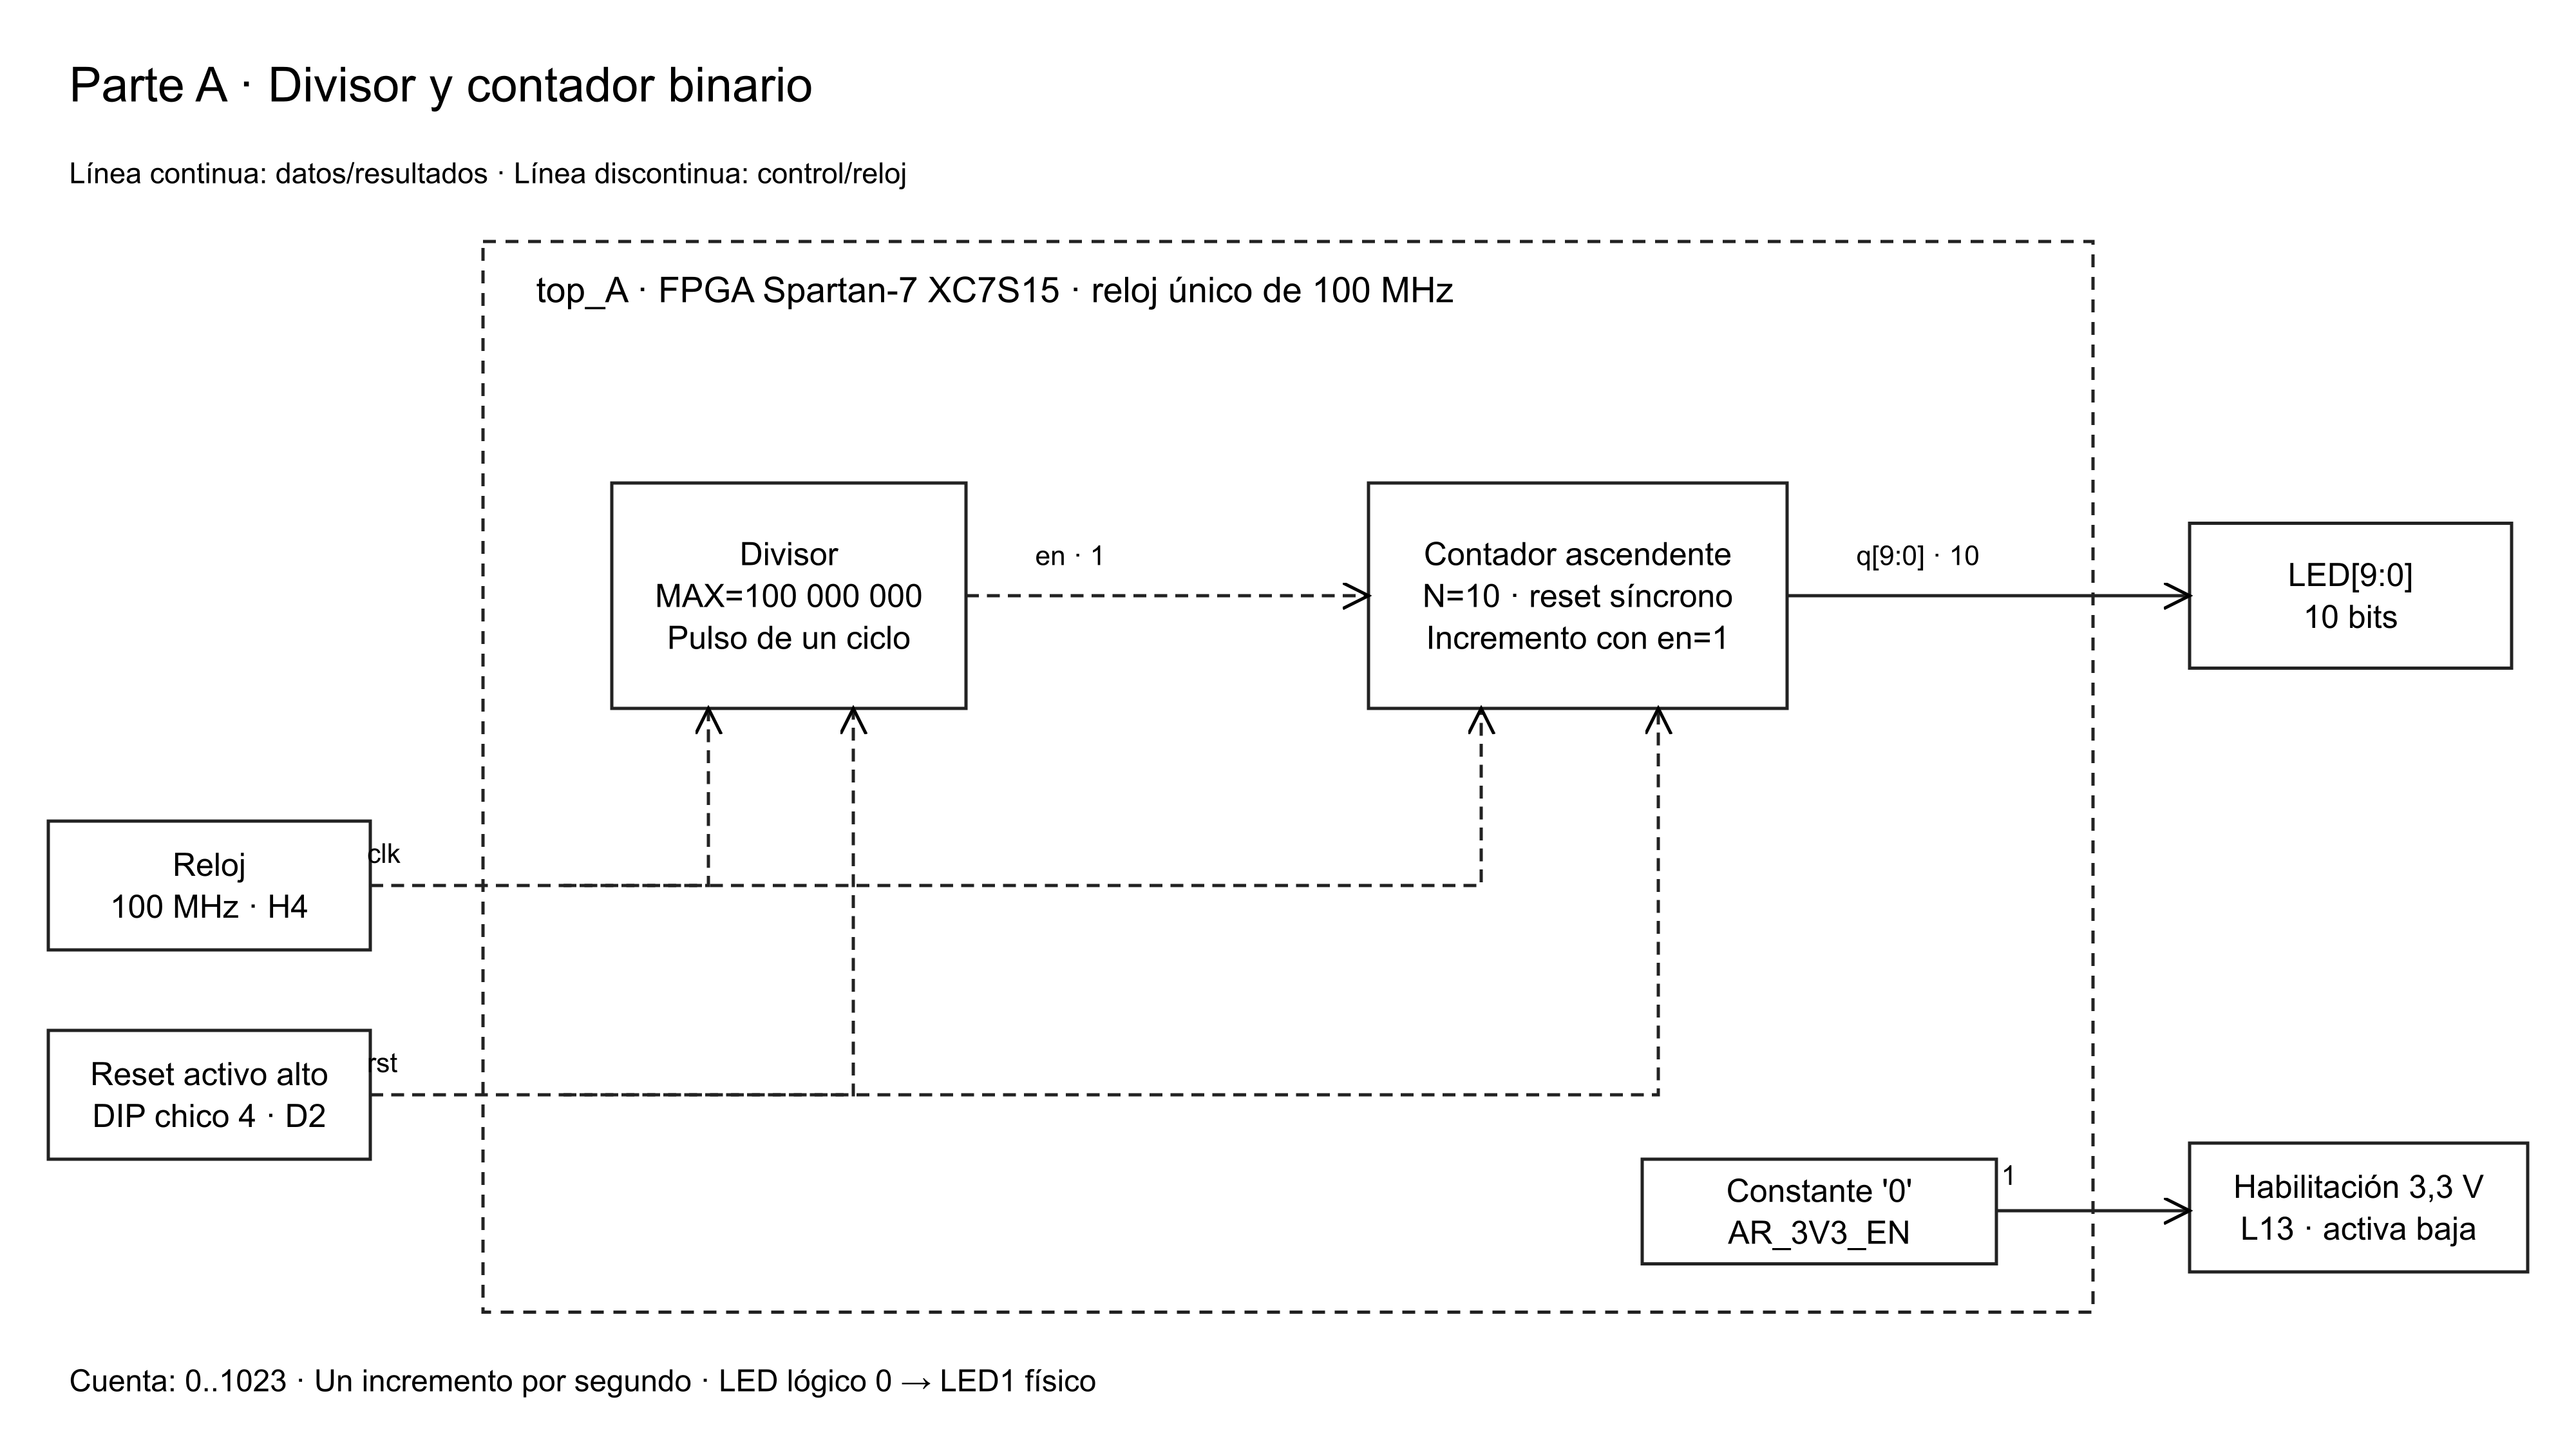
\includegraphics[width=\textwidth]{parte_a_integracion.png}
\caption{Integración de la Parte A: divisor y contador bajo un único reloj, reset común y salida de diez bits hacia los LEDs.}\label{fig:bloquesA}
\end{figure*}

\subsection{Comportamiento temporal esperado}
El pulso \texttt{en} fue especificado como una habilitación de un único ciclo de reloj cada \texttt{MAX} ciclos. Con \texttt{MAX=4}, la separación entre dos activaciones consecutivas fue de cuatro períodos de reloj. Con \texttt{MAX=100\,000\,000} y reloj de 100 MHz, el intervalo fue de un segundo. En un contador binario, cada bit dividió por dos la frecuencia de la señal cuadrada representada por el bit inmediato inferior \cite{cursodiv}. El avance de la cuenta permaneció sujeto a \texttt{en}, no a un flanco de una señal generada por lógica combinacional.

\subsection{Parte B: FSM y diagrama de estados}
Se definieron los estados enumerados \texttt{S\_AND}, \texttt{S\_OR}, \texttt{S\_XOR} y \texttt{S\_ADD}. Cada pulso de habilitación provocó, por especificación, una transición al siguiente estado y, después de \texttt{S\_ADD}, el retorno a \texttt{S\_AND}. El reset se definió con destino \texttt{S\_AND}. Se separaron el registro de estado, la lógica combinacional del próximo estado y la decodificación de la salida \texttt{op}, siguiendo el patrón de tres procesos presentado en el material del curso \cite{cursofsm}. La habilitación se consideró dentro de la lógica de transición o del registro, sin generar un segundo reloj.

\begin{figure}[!t]
\centering
\begin{tikzpicture}[>=Stealth, every node/.style={font=\scriptsize}, st/.style={draw,rounded corners,minimum width=18mm,minimum height=8mm,align=center}, node distance=12mm and 10mm]
\node[st] (a) {S\_AND\\00};
\node[st,right=of a] (b) {S\_OR\\01};
\node[st,below=of b] (c) {S\_XOR\\10};
\node[st,left=of c] (d) {S\_ADD\\11};
\draw[->] (a) -- node[above]{en} (b);
\draw[->] (b) -- node[right]{en} (c);
\draw[->] (c) -- node[below]{en} (d);
\draw[->] (d) -- node[left]{en} (a);
\draw[->] ([xshift=-10mm]a.west) -- node[above]{reset} (a.west);
\path (a) edge[loop above,->] node{sin en} (a)
(b) edge[loop above,->] node{sin en} (b)
(c) edge[loop below,->] node{sin en} (c)
(d) edge[loop below,->] node{sin en} (d);
\end{tikzpicture}
\caption{Diagrama de estados de la FSM implementada. El reset tuvo prioridad sobre la habilitación y estableció S\_AND desde cualquier estado.}\label{fig:fsm}
\end{figure}

\subsection{Parte B: datapath e integración}
El datapath recibió \texttt{A(3:0)}, \texttt{B(3:0)} y \texttt{op(1:0)}. Se definieron las operaciones y la visualización indicadas en la Tabla~\ref{tab:ops}. La suma se representó en cinco bits para conservar el acarreo, mientras que las operaciones lógicas se expresaron en cuatro bits. El divisor de la Parte A fue incorporado como fuente de habilitación para la FSM.

\begin{table}[!t]
\centering\caption{Codificación y salidas de la Parte B}\label{tab:ops}
\begin{tabular}{@{}lllp{0.28\columnwidth}@{}}\toprule
\textbf{op} & \textbf{Estado} & \textbf{Cálculo} & \textbf{Salidas}\\\midrule
00 & AND & \(A\land B\) & LED3:0\\
01 & OR & \(A\lor B\) & LED3:0\\
10 & XOR & \(A\oplus B\) & LED3:0\\
11 & ADD & \(A+B\) & LED4:0\\\bottomrule
\end{tabular}
\end{table}

\begin{figure*}[!t]
\centering
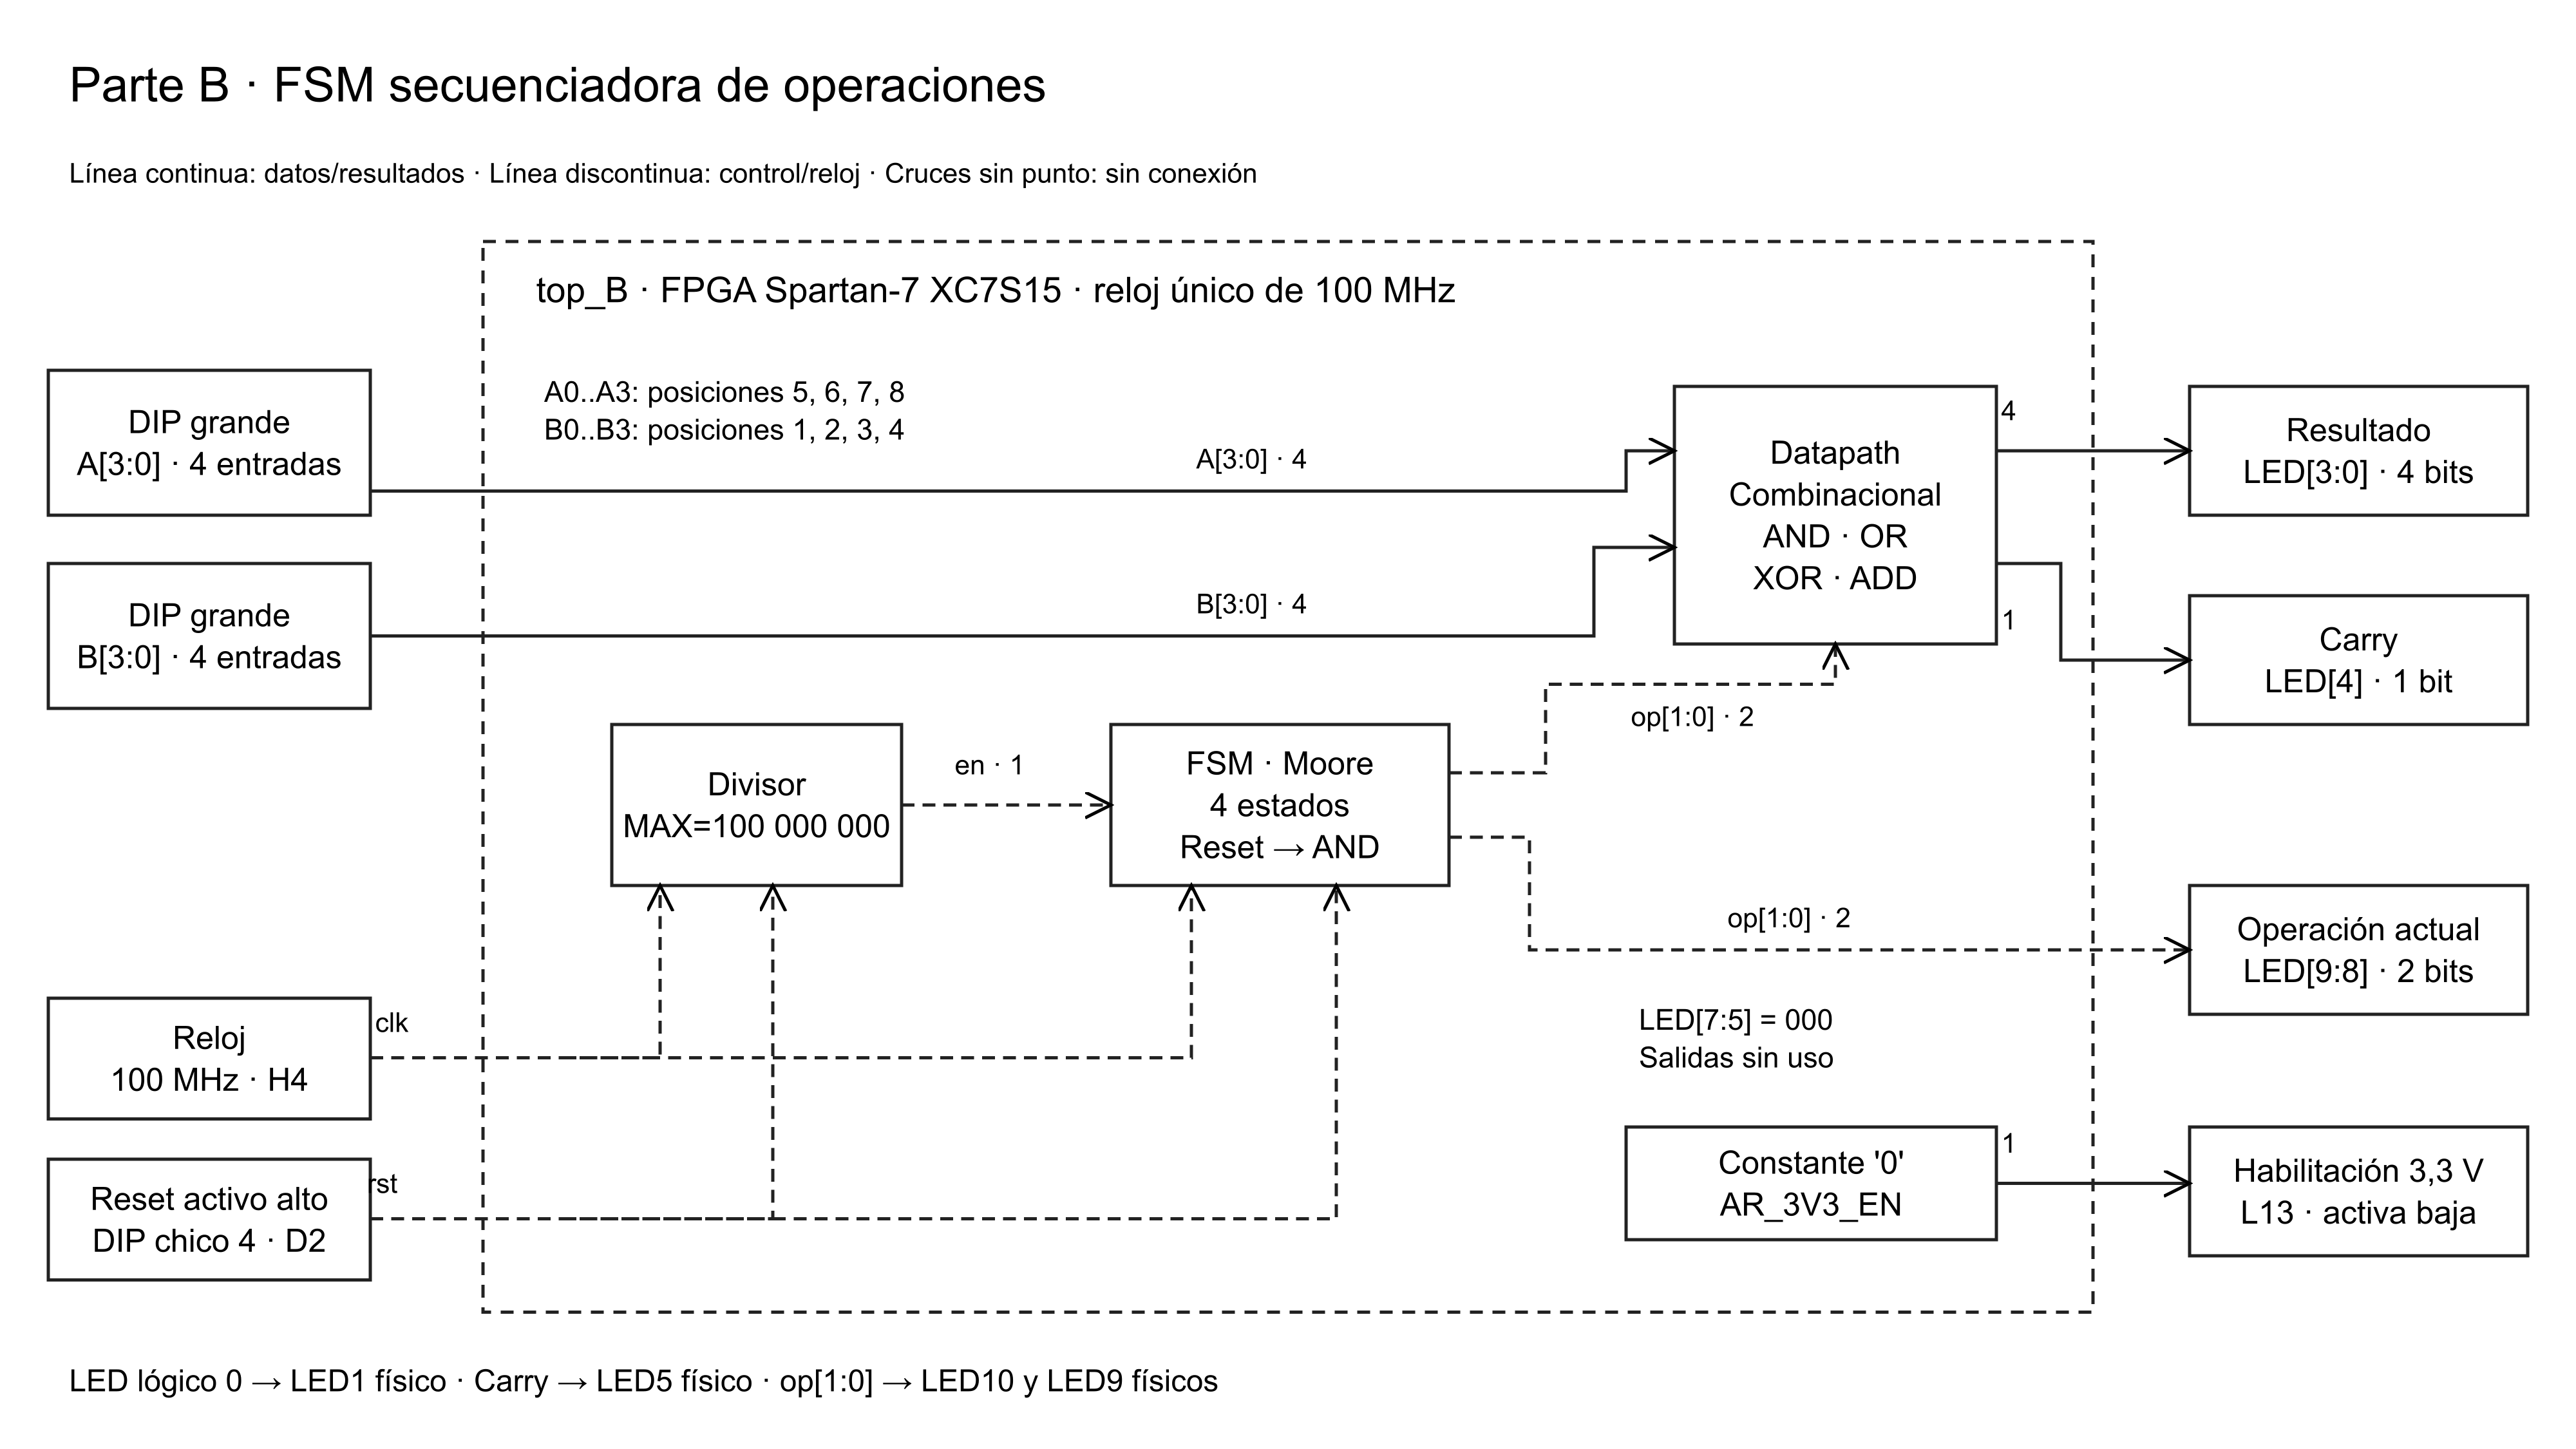
\includegraphics[width=\textwidth]{parte_b_integracion.png}
\caption{Integración de la Parte B: entradas A y B, divisor, FSM, datapath y salidas. El reloj y el reset fueron comunes al divisor y a la FSM; las salidas LED[7:5] fueron fijadas a cero.}\label{fig:bloques}
\end{figure*}

\subsection{Simulación y testbenches}
Para la Parte A se planteó un escenario de prueba con \texttt{MAX=4}, que permitió observar los pulsos sin simular cien millones de ciclos entre habilitaciones. Se fijaron como criterios de verificación la duración de un ciclo de \texttt{en}, su periodicidad, el incremento unitario, el desborde y el reset. En el material de clase se recomendó medir períodos entre eventos con \texttt{now} y utilizar \texttt{assert}; al comparar valores después de un flanco, se propuso un retardo breve para permitir la actualización de los ciclos delta del simulador \cite{cursodiv}. Para la Parte B se establecieron dos recorridos completos de la secuencia, un reset desde un estado distinto de \texttt{S\_AND} y casos de prueba para cada operación, incluida una suma con acarreo. El material de FSM mostró la comparación de salidas esperadas mediante \texttt{assert}, práctica aplicable a la secuencia de \texttt{op} \cite{cursofsm}. La periodicidad de en, la cuenta, el desborde y el reset fueron comprobados mediante assert en la Parte A; la secuencia, la retención, el reset y todos los pares de operandos por operación fueron comprobados mediante assert en la Parte B. Las capturas fueron utilizadas como evidencia visual complementaria.

\subsection{Restricciones e implementación en la placa}
La consigna estableció el reloj de 100 MHz en el pin H4 y requirió la restricción temporal \texttt{create\_clock}. Las entradas y salidas del shield utilizaron el estándar \texttt{LVCMOS33}. Además, la salida \texttt{AR\_3V3\_EN} quedó definida como activa en bajo, con asignación al pin L13 y valor lógico cero para habilitar la alimentación de los dip-switches \cite{consigna}. Se cotejaron las conexiones con el esquema del shield y el XDC maestro de la SEA. El reset se asignó a D2 (A10), posición 4 del DIP chico. Los operandos se agruparon en el DIP grande: A[0:3] en posiciones 5,6,7,8 y B[0:3] en posiciones 1,2,3,4. En la Parte B, A[0:3] se conectó a D9,D8,D7,D6 (A2, B3, A3, A4) y B[0:3] a D13,D12,D11,D10 (H2, H1, B1, B2). Los diez LEDs físicos, LED1 a LED10, se conectaron a LED[0] a LED[9], respectivamente, mediante FPGAIO9 a FPGAIO0. Se completaron síntesis, colocación y ruteo de ambas partes en Vivado 2025.1 para el dispositivo XC7S15FTGB196-1. Se programaron ambas partes por JTAG. La validación física y su registro se documentaron en la sección de resultados.


La Tabla~\ref{tab:dipfinal} resume la asignación física final utilizada en las pruebas.
\begin{table}[!t]
\centering\caption{Asignación final de los DIP-switches}\label{tab:dipfinal}
\begin{tabular}{@{}llll@{}}\toprule
Señal & DIP/posición & Arduino & FPGA\\\midrule
rst & Chico 4 & D2 & A10\\
A0 & Grande 5 & D9 & A2\\
A1 & Grande 6 & D8 & B3\\
A2 & Grande 7 & D7 & A3\\
A3 (MSB) & Grande 8 & D6 & A4\\
B0 & Grande 1 & D13 & H2\\
B1 & Grande 2 & D12 & H1\\
B2 & Grande 3 & D11 & B1\\
B3 (MSB) & Grande 4 & D10 & B2\\\bottomrule
\end{tabular}
\end{table}
